\documentclass{report}
\usepackage[utf8]{inputenc}
\usepackage[english, russian]{babel}
\usepackage{listings}
\usepackage{graphicx}
\usepackage{float}
\graphicspath{{img/}}
\usepackage{amsmath,amsfonts,amssymb,amsthm,mathtools} 
\usepackage{pgfplots}
\usepackage{filecontents}
\usepackage{indentfirst}
\usepackage{eucal}
\usepackage{enumitem}
\frenchspacing

\usepackage{indentfirst} % Красная строка

\usetikzlibrary{datavisualization}
\usetikzlibrary{datavisualization.formats.functions}

\usepackage{amsmath}



% Для листинга кода:
\lstset{ %
language=c++,                 % выбор языка для подсветки (здесь это С)
basicstyle=\small\sffamily, % размер и начертание шрифта для подсветки кода
numbers=left,               % где поставить нумерацию строк (слева\справа)
numberstyle=\tiny,           % размер шрифта для номеров строк
stepnumber=1,                   % размер шага между двумя номерами строк
numbersep=5pt,                % как далеко отстоят номера строк от подсвечиваемого кода
showspaces=false,            % показывать или нет пробелы специальными отступами
showstringspaces=false,      % показывать или нет пробелы в строках
showtabs=false,             % показывать или нет табуляцию в строках
frame=single,              % рисовать рамку вокруг кода
tabsize=2,                 % размер табуляции по умолчанию равен 2 пробелам
captionpos=t,              % позиция заголовка вверху [t] или внизу [b] 
breaklines=true,           % автоматически переносить строки (да\нет)
breakatwhitespace=false, % переносить строки только если есть пробел
escapeinside={\#*}{*)}   % если нужно добавить комментарии в коде
}

\usepackage[left=2cm,right=2cm, top=2cm,bottom=2cm,bindingoffset=0cm]{geometry}
% Для измененных титулов глав:
\usepackage{titlesec, blindtext, color} % подключаем нужные пакеты
\definecolor{gray75}{gray}{0.75} % определяем цвет
\newcommand{\hsp}{\hspace{20pt}} % длина линии в 20pt
\newcommand{\jj}{\righthyphenmin=20 \justifying}
% titleformat определяет стиль
\titleformat{\chapter}[hang]{\Huge\bfseries}{\thechapter\hsp\textcolor{gray75}{|}\hsp}{0pt}{\Huge\bfseries}


% plot
\usepackage{pgfplots}
\usepackage{filecontents}
\usetikzlibrary{datavisualization}
\usetikzlibrary{datavisualization.formats.functions}
 
\begin{document}
\thispagestyle{empty}
\begin{titlepage}
	\noindent \begin{minipage}{0.15\textwidth}
	
\includegraphics[width=\linewidth]{b_logo}
	\end{minipage}
	\noindent\begin{minipage}{0.9\textwidth}\centering
		\textbf{Министерство науки и высшего образования Российской Федерации}\\
		\textbf{Федеральное государственное бюджетное образовательное учреждение высшего образования}\\
		\textbf{~~~«Московский государственный технический университет имени Н.Э.~Баумана}\\
		\textbf{(национальный исследовательский университет)»}\\
		\textbf{(МГТУ им. Н.Э.~Баумана)}
	\end{minipage}
	
	\noindent\rule{18cm}{3pt}
	\newline\newline
	\noindent ФАКУЛЬТЕТ $\underline{\text{«Информатика и системы управления»}}$ \newline\newline
	\noindent КАФЕДРА $\underline{\text{«Программное обеспечение ЭВМ и информационные технологии»}}$\newline\newline\newline\newline\newline\newline\newline\newline\newline\newline\newline
	
	
	\begin{center}
		\noindent\begin{minipage}{1.3\textwidth}\centering
			\Large\textbf{  Отчет по лабораторной работе №1}\newline
			\textbf{по дисциплине "Анализ алгоритмов"}\newline\newline
		\end{minipage}
	\end{center}
	
	\noindent\textbf{Тема} $\underline{\text{Редакционное расстояние}}$\newline\newline
	\noindent\textbf{Студент} $\underline{\text{Варламова Е. А.}}$\newline\newline
	\noindent\textbf{Группа} $\underline{\text{ИУ7-51Б}}$\newline\newline
	\noindent\textbf{Оценка (баллы)} $\underline{\text{~~~~~~~~~~~~~~~~~~~~~~~~~~~}}$\newline\newline
	\noindent\textbf{Преподаватель: } $\underline{\text{Волкова Л.Л.}}$\newline\newline\newline
	
	\begin{center}
		\vfill
		Москва~---~\the\year
		~г.
	\end{center}
\end{titlepage}


\tableofcontents
  
\newpage
\chapter*{Введение}

\addcontentsline{toc}{chapter}{Введение}

Динамическое программирование - это форма вычислений, при которой следующий член вычисляется на основе предыдущего. Простейшим примером применения является вычисление чисел Фибоначчи. Кроме того, динамическое программирование может применяться и в более сложных задачах таких, как проебразование строк из одной в другую. В этом случае задача сводится к вычислению расстояния Левенштейна (редакционного расстояния) - минимального количества опреаций вставки, удаления символа или замены символа один на другой, необходимых для преобразования одной строки в другую. Расстояние Левенштейна применяется в:
\begin{itemize}
\item компьютерной лингвистике для устранения  ошибок в набираемом тексте;
\item в бионформатике для сравнения генов.
\end{itemize}

Поэтому \textbf{целью} данной работы является получение навыка динамического программирования на примере реализации алгоритмов редакционного расстояния. 

Для достижения поставленной цели необходимо решить следующие \textbf{задачи}:
\begin{itemize}
\item изучить алгоритмы расчета редакционного расстояния;
\item реализовать алгоритмы подсчета редакционного расстояния;
\item протестировать реализованные алгоритмы;
\item провести сравнительный анализ реализаций алгоритмов по затраченному процессорному времени и памяти.
\end{itemize}


\chapter{Аналитическая часть}
В данном разделе определяются расстояния Левенштейна и Дамерау-Левенштейна, а также рассматриваются различные алгоритмы вычисления указанных расстояний.

\section{Расстояние Левенштейна}

Для вычисления редакционного расстояния вводятся следующие цены операций:
\begin{itemize}
\item замена одного символа на другой - 1;
\item вставка символа - 1;
\item удаление символа - 1.
\end{itemize}

С учтом этого вводится рекурсивная формула для вычисления расстоянния Левенштейна:
\begin{equation}
\label{eq:LD}
D(s1[1..i], s2[1..j]) = 
\begin{cases}
0,  &\text{i = 0, j = 0}\\
i,  &\text{i > 0, j = 0}\\
j,  &\text{i = 0, j >  0}\\
\min \lbrace \\
\qquad D(s1[1..i], s2[1..j-1]) + 1\\
\qquad D(s1[1..i-1], s2[1..j]) + 1 &\text{i > 0, j > 0}\\
\qquad D(s1[1..i-1], s2[1..j-1]) + 
\begin{cases} 
0, &\text{s1[i] = s2[j]}\\
1, &\text{иначе}\\ 
\end{cases}\\
\rbrace
\end{cases}
\end{equation}

\section{Расстояние Дамерау-Левенштейна}

Дамерау дополнил определение расстояния Левенштейна еще одной операцией, а именно операцией перестановки двух букв местами. Расстояние Дамерау-Левенштейна вычисляется по следующей формуле:

\begin{equation}
\label{eq:DLD}
D(s1[1..i], s2[1..j]) = 
\begin{cases}
0,  &\text{i = 0, j = 0}\\
i,  &\text{i > 0, j = 0}\\
j,  &\text{i = 0, j >  0}\\
\min \lbrace \\
\qquad D(s1[1..i], s2[1..j-1]) + 1\\
\qquad D(s1[1..i-1], s2[1..j]) + 1 &\text{i > 0, j > 0}\\
\qquad D(s1[1..i-1], s2[1..j-1]) + 
\begin{cases} 
0, &\text{s1[i] = s2[j]}\\
1, &\text{иначе}\\ 
\end{cases}\\
\qquad D(s1[1..i-2], s2[1..j-2]) + 1, &\text{если i>1, j>1, s1[i] = s2[j-1], s1[i-1] = s2[j]} \\
\rbrace
\end{cases}
\end{equation}

\section{Нерекусивный алгоритм нахождения расстояния Левенштейна с кэшем в виде матрицы}
Данный алгоритм использует для решения задачи матрицу размером $(m + 1) * (n + 1)$, где $m$ и $n$ - длины двух строк, одну из которых необходимо преобразовать к другой. На каждом шаге работы алгоритма заполняется одна клетка матрицы в соответствии с формулой \ref{eq:LD}. По окончании алгоритма результат будет находиться в последней заполненной клетке.

\section{Нерекусивный алгоритм нахождения расстояния Левенштейна с кэшем в виде 2 строк матрицы}
Данный алгоритм является модификацией предыдущего. Очеивдно, что на кажом шаге алгоритма используются значения из текущей и предыдущей строки матрицы, поэтому достаточно хранить только их, а не всю матрицу.

\section{Рекусивный алгоритм нахождения расстояния Левенштейна}\label{rd}
Данный алгоритм использует для решения формулу \ref{eq:LD}, однако в отличие от прерыдущих является рекурсивным, а значит, для хранения промежуточных результатов используется стек. Кроме того, при этом подходе возникает проблема повторных вычислений, так как функция $D(s1[1..i], s2[1..j])$ будет выполняться несколько раз в разных ветвях дерева.

\section{Рекусивный алгоритм нахождения расстояния Левенштейна с кэшем в виде матрицы}

Данный алгоритм решает проблему повторных вычислений простого рекурсивного алгоритма. При данном подходе вводится матрица размером $(m + 1) * (n + 1)$, содержащая уже вычисленные промежуточные результаты. Изначально матрица инициализируется значениями, которые заведомо не могут быть получены в результате вычислений, например, -1.


\section{Рекусивный алгоритм нахождения расстояния Дамерау-Левенштейна}

Данный алгоритм использует для решения формулу \ref{eq:DLD} и является рекурсивным, а значит, для хранения промежуточных результатов используется стек. Кроме того, при этом подходе возникает проблема повторных вычислений, так как функция $D(s1[1..i], s2[1..j])$ будет выполняться несколько раз в разных ветвях дерева.

\section{Вывод}

В данном разделе были даны определения расстояний Левенштейна и Дамерау-Левенштейна, а также рассмотрены 5 алгоритмов вычисления указанных расстояний.
	
\clearpage

\chapter{Конструкторская часть}
В данном разделе разрабатываются схемы алгоритмов на основе их описания, приведённого в аналитическом разделе.
\section{Схемы алгоритмов}\label{schemes}

На рисунках \ref{fig:mpr1}, \ref{fig:mpr2}, \ref{fig:mpr3} и \ref{fig:mpr4} показаны схемы алгоритма рекурсивного Левенштейна, нерекурсивного алгоритма Левенштейна с кэшем в виде двух строк матрицы, рекурсивного алгоритма Дамерау-Левенштейна и рекурсивного алгоритма с кэшем в виде матрицы соответственно.
\begin{figure}[h!p]\label{recLev}
	\centering
	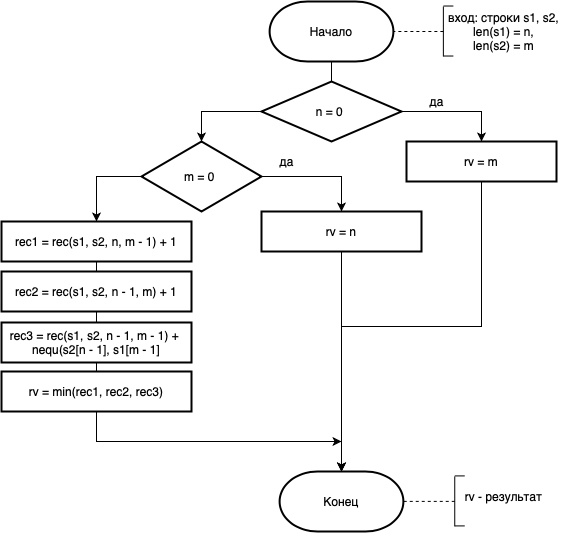
\includegraphics[scale = 0.7]{recLev.drawio.png}
	\caption{Схема рекурсивного алгоритма нахождения расстояния Левенштейна}
	\label{fig:mpr1}
\end{figure}

\begin{figure}[h!p]\label{lev}
	\centering
	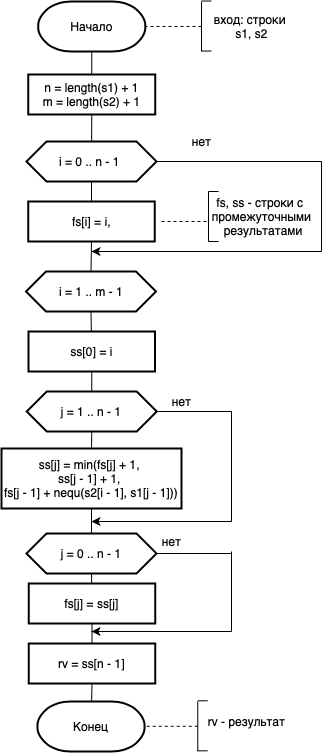
\includegraphics[scale = 0.7]{lev.drawio.png}
	\caption{Схема нерекурсивного алгоритма нахождения расстояния Левенштейна с кэшем в виде двух строк матрицы}
	\label{fig:mpr2}
\end{figure}

\begin{figure}[h!p]\label{recDam}
	\centering
	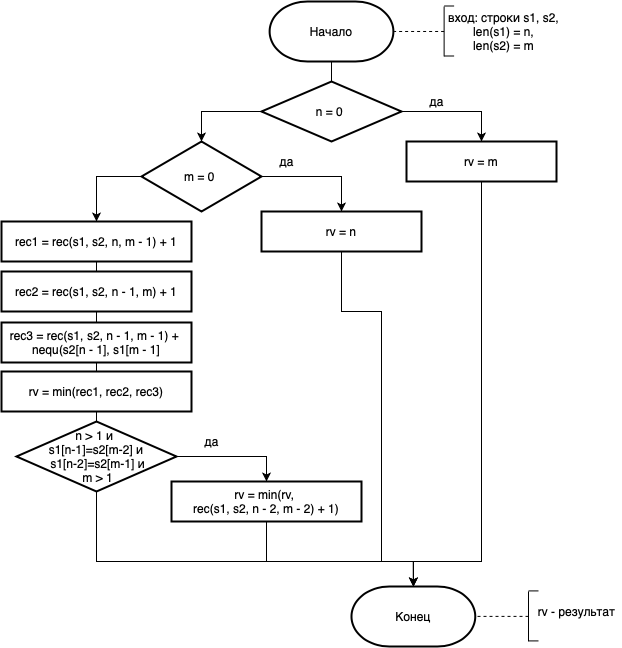
\includegraphics[scale = 0.7]{recDamLev.drawio.png}
	\caption{Схема рекурсивного алгоритма нахождения расстояния Дамерау-Левенштейна}
	\label{fig:mpr3}
\end{figure}
\newpage

\begin{figure}[h!p]\label{recLevMatr}
	\centering
	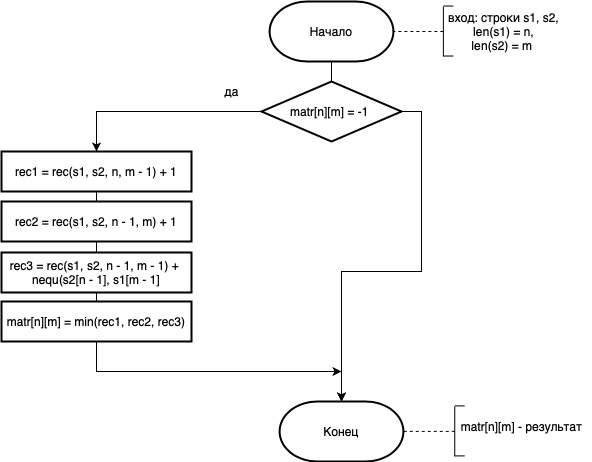
\includegraphics[scale = 0.7]{recLevMatr.drawio.png}
	\caption{Схема рекурсивного алгоритма нахождения расстояния Левенштейна с кэшем в виде матрицы}
	\label{fig:mpr4}
\end{figure}

\section{Вывод}

В данном разделе были построены схемы 4-х алгоритмов нахождения редакционного расстояния на основе их описания, приведённого в аналитической части.
\chapter{Технологическая часть}
В данном разделе приводится реализация алгоритмов, схемы которых были разработаны в конструкторской части. Кроме того, обосновывается выбор технологического стека и проводится тестирование реализованных алгоритмов.
\section{Средства реализации}

В качестве языка программирования был выбран C++ из-за его быстродействия, а среды разработки -- CLion. Время работы алгоритмов было замерено с помощью time.h, функции clock, которая измеряет процессорное время [1].

\section{Реализация алгоритмов}

В листингах 3.1 - 3.4 приведена реализации алгоритмов описанных в \ref{schemes}.

\begin{lstlisting}[label=some-code,caption=Функция для рекурсивного нахождения расстояния Левенштейна с кэшем в виде матрицы,language=C++]
static int _recLevCache(const char * s1, const char * s2, int n, int m, int ** matr)
{
    if (matr[n][m] == -1)
    {
        matr[n][m] = minimum(3,
                             _recLevCache(s1, s2, n, m - 1, matr) + 1,
                             _recLevCache(s1, s2, n - 1, m, matr) + 1,
                             _recLevCache(s1, s2, n - 1, m - 1, matr) + (s1[n - 1] != s2[m - 1]));
    }
    return matr[n][m];
}

int recLevCache(const char * s1, const char * s2)
{
    int n = strlen(s1);
    int m = strlen(s2);

    int **matr = alloc_matrix(n + 1, m + 1);

    for (int i = 0; i < n + 1; i++)
        matr[i][0] = i;
    for (int i = 0; i < m + 1; i++)
        matr[0][i] = i;
    for (int i = 1; i < n + 1; i++)
        for (int j = 1; j < m + 1; j++)
            matr[i][j] = -1;
    int rv = _recLevCache(s1, s2, n, m, matr);
    free_matrix(matr, n, m);
    return rv;
}
\end{lstlisting}
\newpage
\begin{lstlisting}[label=some-code,caption=Функция для нерекурсивного нахождения расстояния Левенштейна с кэшем в виде двух строк матрицы,language=C++]
int levCache(const char * s1, const char * s2)
{
    size_t n = strlen(s1) + 1;
    size_t m = strlen(s2) + 1;

    int *fs = (int *)malloc(n * sizeof(int));
    int *ss = (int *)malloc(n * sizeof(int));
    for (size_t i = 0; i < n; i++)
        fs[i] = i;

    for (size_t i = 1; i < m; i++)
    {
        ss[0] = i;
        for (size_t j = 1; j < n; j++)
            ss[j] = minimum(3,
                        fs[j] + 1,
                        ss[j - 1] + 1,
                        fs[j - 1] + (s2[i - 1] != s1[j - 1]) );
        for (size_t j = 0; j < n; j++) {
            fs[j] = ss[j];
        }
    }

    int rv = ss[n - 1];
    free(fs);
    free(ss);
    return rv;
}
\end{lstlisting}

\begin{lstlisting}[label=some-code,caption=Функция для рекурсивного нахождения расстояния Дамерау-Левенштейна,language=C++]
int _recDamLev(const char * s1, const char * s2, int n, int m)
{
    if (n == 0)
        return m;
    if (m == 0)
        return n;
    int min = minimum(3,
                _recDamLev(s1, s2, n, m - 1) + 1,
                _recDamLev(s1, s2, n - 1, m) + 1,
                _recDamLev(s1, s2, n - 1, m - 1) + (s1[n - 1] != s2[m - 1]));

    if (n > 1 && m > 1 && s1[n - 1] == s2[m - 2] && s1[n - 2] == s2[m - 1])
        min = minimum(2, min, _recDamLev(s1, s2, n - 2, m - 2) + 1);
    return min;
}

int recDamLev(const char * s1, const char * s2)
{
    return _recDamLev(s1, s2, strlen(s1), strlen(s2));
}

\end{lstlisting}
\newpage
\begin{lstlisting}[label=some-code,caption=Функция для рекурсивного нахождения расстояния Левенштейна, language=C++]
int _recLev(const char * s1, const char * s2, int n, int m)
{
    if (n == 0)
        return m;
    if (m == 0)
        return n;

    return minimum(3,
               _recLev(s1, s2, n, m - 1) + 1,
               _recLev(s1, s2, n - 1, m) + 1,
               _recLev(s1, s2, n - 1, m - 1) + (s1[n - 1] != s2[m - 1]));
}

int recLev(const char * s1, const char * s2)
{
    return _recLev(s1, s2, strlen(s1), strlen(s2));
}
\end{lstlisting}

\section{Тестирование}

В таблице~\ref{tbl:test} приведены тесты для функций сортировки.

\begin{table}[h!p]
	\begin{center}
		\caption{\label{tbl:test}Тестирование алгоритмов нахождения расстояния Левенштейна}
		\begin{tabular}{|c|c|c|}
			\hline
			Входные строки & Результат & Ожидаемый результат \\ 
			\hline
			$ckat, kot$ & $2$  & $2$\\\hline
			$abc, defg$  & $4$  & $4$\\\hline
			$abcd, abcd$  & $0$  & $0$\\\hline
		\end{tabular}
	\end{center}
\end{table}

\begin{table}[h!p]
	\begin{center}
		\caption{\label{tbl:test}Тестирование алгоритмов нахождения расстояния Дамерау-Левенштейна}
		\begin{tabular}{|c|c|c|}
			\hline
			Входные строки & Результат & Ожидаемый результат \\ 
			\hline
			$ckat, kot$ & $2$  & $2$\\\hline
			$abc, defg$  & $4$  & $4$\\\hline
			$abcd, abcd$  & $0$  & $0$\\\hline
			$abcd, badc$  & $2$  & $2$\\\hline
		\end{tabular}
	\end{center}
\end{table}

Все тесты пройдены успешно.

\section{Вывод}

В данном разделе были реализованы 4 алгоритма нахождения редакционного расстояния с помощью выбранных средств разработки. Кроме того, реализованные алгоритмы были протестированы.

\chapter{Исследовательская часть}
В эданном разделе проводится сравненительный анализ реализованных алгоритмов по процессорному времени и по затарчиваемой памяти.
\section{Технические характеристики}

Все нижепреведенные замеры времени проведены на процессоре: Intel Core i5, 1,4 GHz, 4‑ядерный.

\section{Время выполнения реализаций алгоритмов}

Для сравнительного анализа времени выполнения реализаций алгоритмов проведен эксперимент. Для замеров были сформированы строки, с суммарной длиной, варьирующейся от 6 до 24 включительно с шагом 2.

Время измерялось 10 раз для каждой пары строк, после усреднялось. Время на графиках (рис. \ref{fig:mpr5}) представлено в милисекундах. 

\begin{figure}[h!p]\label{1}
	\centering
	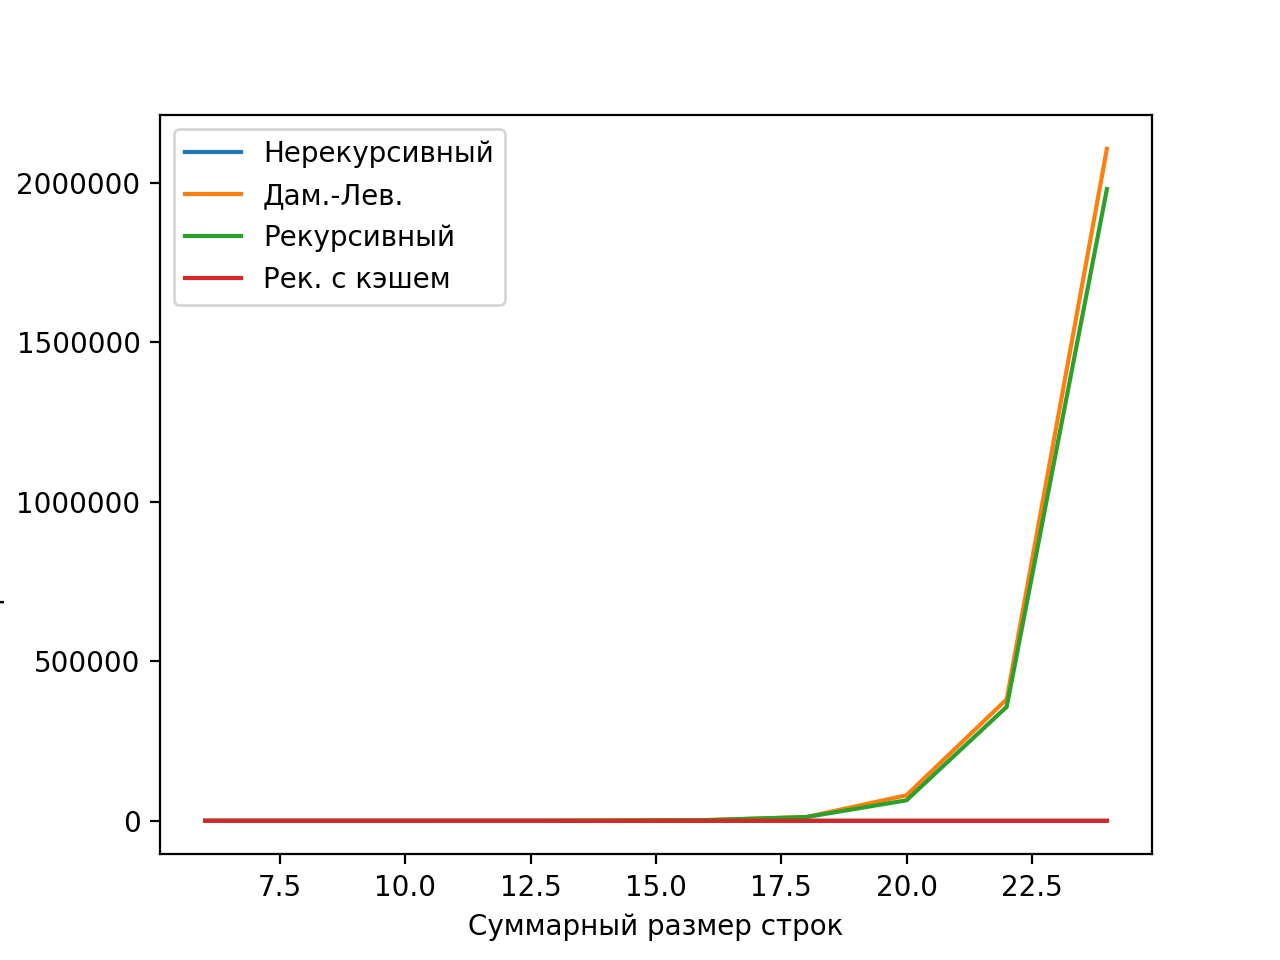
\includegraphics[scale = 0.85]{gr.png}
	\caption{Зависимость времени от суммарной длины строк}
	\label{fig:mpr5}
\end{figure}

\newpage

Время для всех реализаций представлено в таблице \ref{tb:times}.

\begin{table}[h!p]
	\begin{center}
		\caption{\label{tbl:test}Зависимость затрачиваемого процессорного времени от суммарной длины строк для 4 алгоритмов}
		\label{tb:times}
		\begin{tabular}{|c|c|c|c|c|}
			\hline
			Суммарная длина строк & Нерек. & Дам.-Лев. & Рек. & Рек. с кэшем  \\ 
			\hline
            6 & 2.70 & 1.20 & 1.20 & 2.20  \\ 
            \hline
            8 & 1.00 & 4.80 & 3.30 & 2.20  \\ 
            \hline
            10 & 1.30 & 16.70 & 15.60 & 2.20  \\ 
            \hline
            12 & 1.10 & 87.30 & 86.90 & 2.80  \\ 
            \hline
            14 & 1.50 & 475.10 & 451.30 & 4.80  \\ 
            \hline
            16 & 2.00 & 2652.20 & 2650.30 & 4.70  \\ 
            \hline
            18 & 3.00 & 14573.00 & 16364.90 & 6.20  \\ 
            \hline
            20 & 2.10 & 73969.10 & 68309.80 & 11.30  \\ 
            \hline
            22 & 2.60 & 375357.00 & 348323.20 & 5.10  \\ 
            \hline
            24 & 4.70 & 2033420.40 & 1913548.70 & 6.00  \\ 
            \hline
		\end{tabular}
	\end{center}
\end{table}

\section{Оценка затрачиваемой памяти}

В последующих подразделах n - длина первой строки, m - длина второй строки.

\subsection{Рекурсивный алгоритм нахождения расстояния Левенштейна}\label{recmem}
Рассмотрим рекурсивный алгоритм нахождения расстояния Левенштейна.
Максимальная высота дерева будет равна сумме длин двух строк.\newline
На стеке будет выделено максимум: $40 * (n + m) + С$ байт.\newline
На куче память не выделяется.\newline
Итого будет выделено максимум:  $40 * (n + m) + С$ байт.

\subsection{Рекурсивный алгоритм нахождения расстояния Левенштейна с кэшем в виде матрицы}
В данном алгоритме дерево будет такой же высоты как и в \ref{recmem}. Но в данной реализации также выделяется матрица размером n * m на куче.\newline
На стеке будет выделено максимум: $40 * (n + m)$ байт.\newline
На куче будет выделено: $(n * m) * 4 $ байт.\newline
Итого будет выделено максимум:  $40 * (n + m) + (n * m) * 4$ байт.

\subsection{Нерекурсивный алгоритм нахождения расстояния Левенштейна с кэшем в виде 2 строк матрицы}
В данной реализации выделяется 2 строки матрицы длиной m.
На стеке всегда будет выделенно одно и то же количество памяти, так так реализация нерекурсивная.\newline
На куче будет выделено: $m * 2 * 4$ байт.\newline
Итого будет выделено максимум:  $8 * m + С$ байт.

\subsection{Рекурсивный алгоритм нахождения расстояния Дамерау-Левенштейна}
Данная реализация будет занимать столько же памяти сколько и реализация рекусивного алгоритма нахождения расстояния Левенштейна (\ref{recmem}), так как максимальная высота дерева будет одинаковой в обоих случаях, реализации используют одинаковое количество локальных переменных и переменных, поступающих на стек в виде аргументов.


\section{Вывод}

В результате эксперимента можно сделать вывод, что нерекурсивная реализация алгоритма нахождения расстояния Левенштейна с кэшем в виде двух строк матрицы является самой эффективной по процессорному времени и затрачиваемой памяти. Рекурсивный алгоритм с кэшэм в виде матрицы менее эффективен по памяти, чем нерекурсивный, однако значительно быстрее, чем обычный рекусивный (и рекурсивный Дамерау-Левенштейна).


\chapter*{Заключение}
\addcontentsline{toc}{chapter}{Заключение}

В рамках данной лабораторной работы были решены следующие задачи:

\begin{itemize}
	\item изучены 4 алгоритма расчета редакционного расстояния;
	\item реализованы 4 алгоритма расчета редакционного расстояния;
	\item протестированы реализованные алгоритмы;
	\item проведён сравнительный анализ алгоритмов по затраченному процессорному времени и памяти.
\end{itemize}
Поставленная цель, состоящая в получении навыка динамического программирования на примере реализации алгоритмов редакционного расстояния, достигнута.

\chapter*{Литература}
\addcontentsline{toc}{chapter}{Литература}
\begin{enumerate}
	\item Стандартная функция clock(), измеряющая процессорное время [Электронный ресурс]. Режим доступа: https://en.cppreference.com/w/cpp/chrono/c/clock. Дата обращения: 24.09.2021
\end{enumerate}


\end{document}
